%%%%%%%%%%%%%%%%%%%%%%%%%
\section{Introduction}
\label{sec:Introduction}
%%%%%%%%%%%%%%%%%%%%%%%%%

Modular Self-Reconfigurable Robots (MSRR) have been proposed as one method to create general purpose robotic systems of arbitrary complexity in an autonomous way. MSRR systems generally can be thought of as consisting of individual \textbf{modules}, which connect to either other active modules or passive modular elements, through standardized \textbf{connectors} to create a specific \textbf{configuration} in order to accomplish a designated task. Much of the work in the MSRR field has focused either on the preliminary development of novel hardware systems, or general purpose algorithms on simulated systems. Few MSRR systems remain under active development long enough in order to develop practical algorithms that can accomplish tasks while operating under the constraints of actual existing hardware. This paper is focused on implementing and analyzing three separate practical partially decentralized "behaviors" with a set of 3D M-Block modules.

\begin{figure}[t]
	\centering
	\begin{subfigure}[b]{1.6 in}
		%	\resizebox{.48\linewidth}{0.6 in}
		%	{
		\includegraphics[width=.9\linewidth]{Figures/mTagsCover.png}
		%	}
		\subcaption{}
	\end{subfigure}
	~
	\begin{subfigure}[b]{1.5 in}
		
		
		\resizebox{1.5 in}{1.25 in}
		{
			\begin{tikzpicture}[x=(220:1cm), y=(-40:1cm), z=(90:0.707cm)]
			
			%%
%this code is from...
\setcounter{x}{0}%
\setcounter{y}{0}%
\setcounter{z}{0}%

% The angles of x,y,z-axes
\newcommand\xaxis{210}
\newcommand\yaxis{-30}
\newcommand\zaxis{90}

% The top side of a cube
\newcommand\topside[3]{
	\fill[fill=yellow, draw=black,shift={(\xaxis:#1)},shift={(\yaxis:#2)},
	shift={(\zaxis:#3)}] (0,0) -- (30:1) -- (0,1) --(150:1)--(0,0);
}

% The left side of a cube
\newcommand\leftside[3]{
	\fill[fill=red, draw=black,shift={(\xaxis:#1)},shift={(\yaxis:#2)},
	shift={(\zaxis:#3)}] (0,0) -- (0,-1) -- (210:1) --(150:1)--(0,0);
}

% The right side of a cube
\newcommand\rightside[3]{
	\fill[fill=blue, draw=black,shift={(\xaxis:#1)},shift={(\yaxis:#2)},
	shift={(\zaxis:#3)}] (0,0) -- (30:1) -- (-30:1) --(0,-1)--(0,0);
}

% The cube 
\newcommand\cube[3]{
	\topside{#1}{#2}{#3} \leftside{#1}{#2}{#3} \rightside{#1}{#2}{#3}
}

\newcommand\ArrowNE[3]
{
	\node at (#1+0.5, #2+0.5, #3) 
%	\node at (#1, #2, #3) 
	{
		\begin{tikzpicture}
		\draw[->, thick, >={Stealth[round]}, line width=0.4mm] (0.3,0) -- (-0.3,0);
		\end{tikzpicture}};
		
}

\newcommand\ArrowNL[3]
{
	\node at (#1+1, #2+0.5, #3-0.5) 
	%	\node at (#1, #2, #3) 
	{
		\begin{tikzpicture}
		\draw[->, thick, >={Stealth[round]}, line width=0.4mm] (0.16,0.16) -- (-0.16,-0.16);
		\end{tikzpicture}};
	
}

\newcommand\ArrowNR[3]
{
	\node at (#1+0.5, #2+1, #3-0.5) 
	%	\node at (#1, #2, #3) 
	{
		\begin{tikzpicture}
		\draw[->, thick, >={Stealth[round]}, line width=0.4mm] (0.16,0.16) -- (-0.16,-0.16);
		\end{tikzpicture}};
	
}

\newcommand\ArrowNW[3]
{
	\node at (#1+0.5, #2+0.5, #3) 
%	\node at (#1, #2, #3) 
	{
		\begin{tikzpicture}
		\draw[->, thick, >={Stealth[round]}, line width=0.4mm] (0,0.3) -- (0,-0.3);
		\end{tikzpicture}};
	
}

\newcommand\ArrowSW[3]
{
	\node at (#1+0.5, #2+0.5, #3) 
%	\node at (#1, #2, #3) 
	{
		\begin{tikzpicture}
		\draw[<-, thick, >={Stealth[round]}, line width=0.4mm] (0.3,0) -- (-0.3,0);
		\end{tikzpicture}};
	
}

\newcommand\ArrowSE[3]
{
	\node at (#1+0.5, #2+0.5, #3) 
%	\node at (#1, #2, #3) 
	{
		\begin{tikzpicture}
		\draw[<-, thick, >={Stealth[round]}, line width=0.4mm] (0,0.3) -- (0,-0.3);
		\end{tikzpicture}};
	
}

% Definition of \planepartition
% To draw the following plane partition, just write \planepartition{ {a, b, c}, {d,e} }.
%  a b c
%  d e
\newcommand\planepartition[1]{
	\setcounter{x}{-1}
	\foreach \a in {#1} {
		\addtocounter{x}{1}
		\setcounter{y}{-1}
		\foreach \b in \a {
			\addtocounter{y}{1}
			\setcounter{z}{-1}
			\foreach \c in {0,...,\b} {
				\addtocounter{z}{1}
				\ifthenelse{\c=0}{\setcounter{z}{-1},\addtocounter{y}{0}}{
					\cube{\value{x}}{\value{y}}{\value{z}}}
			}
		}
	}
}


%%\begin{tikzpicture}[x=(220:1cm), y=(-40:1cm), z=(90:0.707cm)]
	%\planepartition{{0,0,1},{1,1,1},{1,0,0},{1,0,1}};
\foreach \m [count=\y] in {{1,1,1,1},{1,1,1},{1,1,1,1},{1,1,1}}{
	\foreach \n [count=\x] in \m {
		\ifnum \n>0
		\foreach \z in {1,...,\n}{
			\draw [fill=blue!30] (\x+1,\y,\z) -- (\x+1,\y+1,\z) -- (\x+1, \y+1, \z-1) -- (\x+1, \y, \z-1) -- cycle;
			\draw [fill=blue!40] (\x,\y+1,\z) -- (\x+1,\y+1,\z) -- (\x+1, \y+1, \z-1) -- (\x, \y+1, \z-1) -- cycle;
			\draw [fill=blue!10] (\x,\y,\z)   -- (\x+1,\y,\z)   -- (\x+1, \y+1, \z)   -- (\x, \y+1, \z) -- cycle;  
		}
	
		\fi
	}
}   

\foreach \m [count=\y] in {{0,0,0,1}, {0,0,0}} {
	\foreach \n [count=\x] in \m {
		\ifnum \n>0
		\foreach \z in {1,...,\n}{
			\draw [fill=green!30] (\x+1,\y,\z) -- (\x+1,\y+1,\z) -- (\x+1, \y+1, \z-1) -- (\x+1, \y, \z-1) -- cycle;
			\draw [fill=green!40] (\x,\y+1,\z) -- (\x+1,\y+1,\z) -- (\x+1, \y+1, \z-1) -- (\x, \y+1, \z-1) -- cycle;
			\draw [fill=green!10] (\x,\y,\z)   -- (\x+1,\y,\z)   -- (\x+1, \y+1, \z)   -- (\x, \y+1, \z) -- cycle;  
		}
		
		\fi
	}
}   

\ArrowNW{1}	{3}	{1};

\foreach \m [count=\y] in {{0,0,0,0},{0,0,0},{0,0,0,0},{2,0,0}}{
	\foreach \n [count=\x] in \m {
		\ifnum \n>0
		\foreach \z in {1,...,\n}{
			\draw [fill=orange!30] (\x+1,\y,\z) -- (\x+1,\y+1,\z) -- (\x+1, \y+1, \z-1) -- (\x+1, \y, \z-1) -- cycle;
			\draw [fill=orange!40] (\x,\y+1,\z) -- (\x+1,\y+1,\z) -- (\x+1, \y+1, \z-1) -- (\x, \y+1, \z-1) -- cycle;
			\draw [fill=orange!10] (\x,\y,\z)   -- (\x+1,\y,\z)   -- (\x+1, \y+1, \z)   -- (\x, \y+1, \z) -- cycle;  
		}
		
		\fi
	}
}  

\foreach \m [count=\y] in {{0},{0},{0},{0,1,1}}{
	\foreach \n [count=\x] in \m {
		\ifnum \n>0
		\foreach \z in {1,...,\n}{
			\draw [fill=blue!30] (\x+1,\y,\z) -- (\x+1,\y+1,\z) -- (\x+1, \y+1, \z-1) -- (\x+1, \y, \z-1) -- cycle;
			\draw [fill=blue!40] (\x,\y+1,\z) -- (\x+1,\y+1,\z) -- (\x+1, \y+1, \z-1) -- (\x, \y+1, \z-1) -- cycle;
			\draw [fill=blue!10] (\x,\y,\z)   -- (\x+1,\y,\z)   -- (\x+1, \y+1, \z)   -- (\x, \y+1, \z) -- cycle;  
		}
		
		\fi
	}
} 

\foreach \m [count=\y] in {{0},{0},{0},{1,0,0}}{
	\foreach \n [count=\x] in \m {
		\ifnum \n>0
		\foreach \z in {1,...,\n}{
		%	\draw [fill=blue!30] (\x+1,\y,\z) -- (\x+1,\y+1,\z) -- (\x+1, \y+1, \z-1) -- (\x+1, \y, \z-1) -- cycle;
			\draw [fill=blue!40] (\x,\y+1,\z) -- (\x+1,\y+1,\z) -- (\x+1, \y+1, \z-1) -- (\x, \y+1, \z-1) -- cycle;
		%	\draw [fill=blue!10] (\x,\y,\z)   -- (\x+1,\y,\z)   -- (\x+1, \y+1, \z)   -- (\x, \y+1, \z) -- cycle;  
		}
		
		\fi
	}
} 
		"x" "y" "z"

\ArrowNR{4} {1}	{1};
\ArrowNL{4} {1}	{1};

\ArrowNR{4} {3}	{1};
\ArrowNL{4} {3}	{1};

\ArrowNR{3} {4}	{1};
\ArrowNL{3} {4}	{1};

\ArrowNR{1} {4}	{1};
\ArrowNR{2} {4}	{1};

\ArrowNL{3} {2}	{1};

\ArrowSW{1}	{1}	{1};
\ArrowSW{2}	{1}	{1};
\ArrowSW{3}	{1}	{1};
\ArrowSW{4}	{1}	{1};


\ArrowNW{1}	{2}	{1};
\ArrowSW{2}	{2}	{1};
\ArrowNW{3}	{2}	{1};

\ArrowNW{2}	{3}	{1};
\ArrowNE{3}	{3}	{1};
\ArrowNE{4}	{3}	{1};

%\ArrowNW{1}	{4}	{1};
\ArrowSW{2}	{4}	{1};
\ArrowNW{3}	{4}	{1};

			
			\end{tikzpicture}
		}
		
		\subcaption{}
	\end{subfigure}
	
%	\centering
	\begin{subfigure}[b]{\linewidth}

		%	{
		\centering
		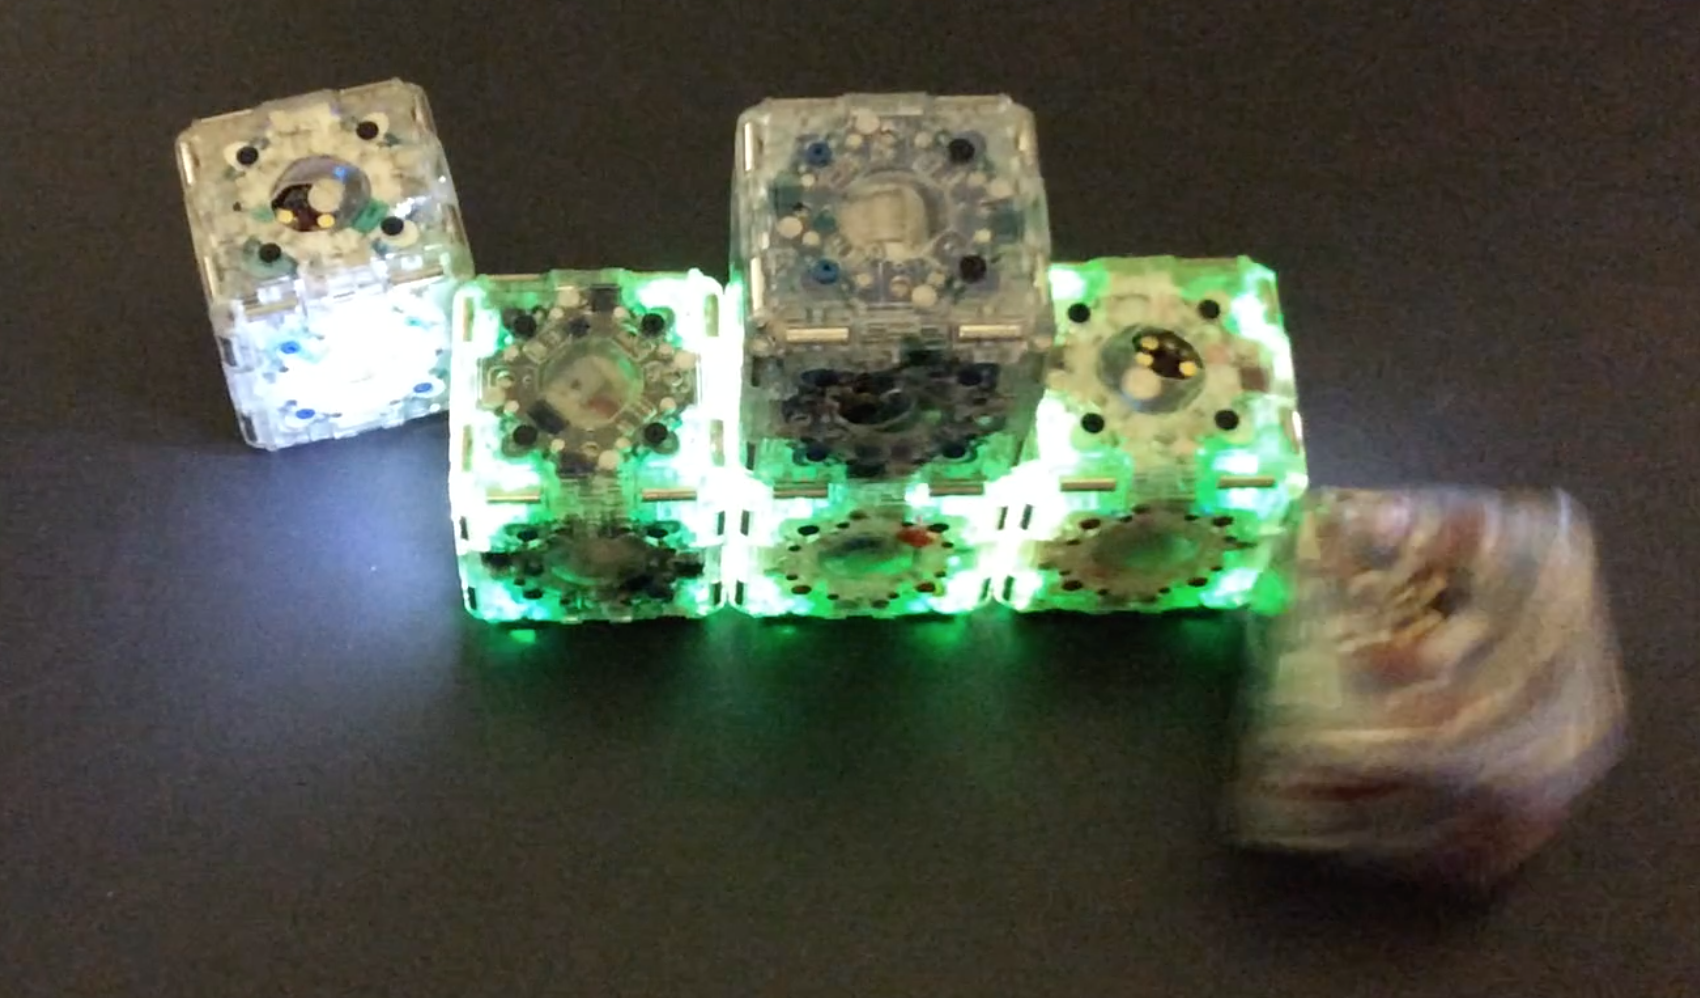
\includegraphics[width=.92\linewidth]{figures/ActualLine_3.png}
		%	}

	\end{subfigure}
	
	
	\caption{This figure shows a sample of several largely decentralized behaviors implemented with a lattice based MSRR system and described in this work. (a) Shows a photo of an active module connected to a passive module which contains a Magnetic Fiducial  (b) Demonstrates an abstraction of these embedded commands as "arrows" which a module that is attempting to follow a path would move along. In this example, the module shown in \emph{orange} would arrive at the \emph{green} module after successfully implementing the path following behavior. (c) Shows a screen-shot from a group of modules implementing the behavior to turn into a single line, with the modules lighted in green, forming the desired line.}
	
	\label{fig:intro}
\end{figure}

The conceptually simplest framework for controlling thousands or millions of individual modular robots is to have a centralized authority which dictates every move to each robot. However these systems suffer from practical problems maintaining the required number of communication links and a general lack of robustness to disturbances. One approach is to develop ingrained "behaviors" or simple decentralized algorithms which each module can implement independently in the (potentially temporary) absence of centralized commutations. When developing these behaviors, the type of sensor feedback, and potential availability and type of local communication are important to determining the possible complexity of possible behaviors. This work focuses on modules which have information only about their direct neighbors,global input from a stimulus source(i.e. Light), knowledge about gravity, and occasional wireless communication. The behaviors that we introduce are as follows:

\begin{itemize}
	\item \textit{Path following}: The goal of this behavior is guide mobile modules to follow paths described by fiducials embedded in in adjacent modules' lattice connection points. This behavior requires that  each module can determine from each of its neighbor connection interfaces a desired direction relative to its current absolute location that the module should move towards. The simplest implementation of this path following behavior involves passive hard-coded "arrow tags" in a lattice of passive modules, similar to arrows embedded along a road, as in Figure~\ref{fig:intro}a-b. Path following behavior is then extended to modules which have connection face identities which are globally uniquely defined, and which contain some embedded "direction" or ability to determine the relative connection angle. Modules can then receive a mapping of ID numbers and "directions", and then can follow a virtually created path along a configuration of modules. A path could be defined along the surface of a large partially assembled aggregate of modules to guide modules to desired attachment points, similar to how optimization technique following gradient descent paths to reach a goal.
	\item \textit{Line formation}: This behavior attempts to turn any arbitrary three-dimensional configuration of modules into a single horizontal line, ready to turn into a new shape on demand. This behavior can be implemented in several ways, but in this work each modules uses knowledge of its direct neighbors, and very simple communication between the faces of adjacent modules. These communications can be as simple as a binary "connect here" or "keep moving," light based symbol or can incorporate the path following behavior to optimize the movement efficiency (i.e. assembly speed) for a group of modules.
	\item \textit{Light gradient}: This goal of this behavior is to implement essentially a Braitenberg phototaxis~\ behavior for modular robots, i.e. aggregating robots towards or away from a light source. In implementation of the behavior presented in this work, the modules begin un-connected to a lattice and continue to move towards light until they reach a specific "goal" structure defined by a specific aggregate of modules, which ensures that aggregation of many modules doesn't lead to smaller scattered groups of modules.
\end{itemize}

This work is implemented and experimentally validated through a set of 12 3D M-Block modular robots; which are one of the few MSRR systems capable of three-dimensional reconfiguration according to a generalized 3D lattice reconfiguration model. These ~50mm cubic modules use pulses of angular momentum and temporary magnetic hinges in order to implement lattice reconfiguration according to the Pivoting Cube Model (PCM). The M-Blocks were originally presented as two-dimensional system in 2013~\cite{RomanishinRus-IROS13} and extended to three dimensions in 2015~\cite{Romanishin20153d}. In order to facilitate the implementation of the three previously described behaviors, the 3D M-Blocks are further extended in this work to include a novel type of magnetic bar-code like tag to detect information about their neighbors. This new tag, called the \tagNamePlural, provides globally unique identification codes for each face of a collection of modules. \textit{\TagNamePlural} include relative orientation of the connection (e.g. North, south east, west) between the reading module and are implemented through a standardized configuration of passively embedded inexpensive permanent magnets which can easily be placed into any modular connection interface. These tags are completely passive, so a system of modules can still accurately determine its global configuration even if large numbers of the modules are inactive, either because they are passive, or due to individual module failure.

The remainder of the paper is organized as follows: Section~\ref{sec:RelatedWork} gives an overview of related work that pertains to modular robots with a focus on how existing MSRR systems identify and encode physical configuration information through their connectors. Next, Section~\ref{sec:Hardware} presents the technical details of the proposed \tagNamePlural~system for determining neighbor connection information and then attempts to characterize their functionality and discusses current limitations and potential future extensions. Next, Section ~\ref{sec:Behaviors} presents the detailed algorithms which implement the three behaviors, (1) Path following: (2) Line formation and (3) Light Aggregation, while Section~\ref{sec:Experiments} presents and analyzes experiments implementing these three algorithms. Finally, Section~\ref{sec:Discussion} attempts to help illustrate several of the challenges and requirements for eventually applying these behaviors to future systems with millions of modules.


%\begin{figure}[htb]
%
%	%%
%this code is from...
\setcounter{x}{0}%
\setcounter{y}{0}%
\setcounter{z}{0}%

% The angles of x,y,z-axes
\newcommand\xaxis{210}
\newcommand\yaxis{-30}
\newcommand\zaxis{90}

% The top side of a cube
\newcommand\topside[3]{
	\fill[fill=yellow, draw=black,shift={(\xaxis:#1)},shift={(\yaxis:#2)},
	shift={(\zaxis:#3)}] (0,0) -- (30:1) -- (0,1) --(150:1)--(0,0);
}

% The left side of a cube
\newcommand\leftside[3]{
	\fill[fill=red, draw=black,shift={(\xaxis:#1)},shift={(\yaxis:#2)},
	shift={(\zaxis:#3)}] (0,0) -- (0,-1) -- (210:1) --(150:1)--(0,0);
}

% The right side of a cube
\newcommand\rightside[3]{
	\fill[fill=blue, draw=black,shift={(\xaxis:#1)},shift={(\yaxis:#2)},
	shift={(\zaxis:#3)}] (0,0) -- (30:1) -- (-30:1) --(0,-1)--(0,0);
}

% The cube 
\newcommand\cube[3]{
	\topside{#1}{#2}{#3} \leftside{#1}{#2}{#3} \rightside{#1}{#2}{#3}
}

\newcommand\ArrowNE[3]
{
	\node at (#1+0.5, #2+0.5, #3) 
%	\node at (#1, #2, #3) 
	{
		\begin{tikzpicture}
		\draw[->, thick, >={Stealth[round]}, line width=0.4mm] (0.3,0) -- (-0.3,0);
		\end{tikzpicture}};
		
}

\newcommand\ArrowNL[3]
{
	\node at (#1+1, #2+0.5, #3-0.5) 
	%	\node at (#1, #2, #3) 
	{
		\begin{tikzpicture}
		\draw[->, thick, >={Stealth[round]}, line width=0.4mm] (0.16,0.16) -- (-0.16,-0.16);
		\end{tikzpicture}};
	
}

\newcommand\ArrowNR[3]
{
	\node at (#1+0.5, #2+1, #3-0.5) 
	%	\node at (#1, #2, #3) 
	{
		\begin{tikzpicture}
		\draw[->, thick, >={Stealth[round]}, line width=0.4mm] (0.16,0.16) -- (-0.16,-0.16);
		\end{tikzpicture}};
	
}

\newcommand\ArrowNW[3]
{
	\node at (#1+0.5, #2+0.5, #3) 
%	\node at (#1, #2, #3) 
	{
		\begin{tikzpicture}
		\draw[->, thick, >={Stealth[round]}, line width=0.4mm] (0,0.3) -- (0,-0.3);
		\end{tikzpicture}};
	
}

\newcommand\ArrowSW[3]
{
	\node at (#1+0.5, #2+0.5, #3) 
%	\node at (#1, #2, #3) 
	{
		\begin{tikzpicture}
		\draw[<-, thick, >={Stealth[round]}, line width=0.4mm] (0.3,0) -- (-0.3,0);
		\end{tikzpicture}};
	
}

\newcommand\ArrowSE[3]
{
	\node at (#1+0.5, #2+0.5, #3) 
%	\node at (#1, #2, #3) 
	{
		\begin{tikzpicture}
		\draw[<-, thick, >={Stealth[round]}, line width=0.4mm] (0,0.3) -- (0,-0.3);
		\end{tikzpicture}};
	
}

% Definition of \planepartition
% To draw the following plane partition, just write \planepartition{ {a, b, c}, {d,e} }.
%  a b c
%  d e
\newcommand\planepartition[1]{
	\setcounter{x}{-1}
	\foreach \a in {#1} {
		\addtocounter{x}{1}
		\setcounter{y}{-1}
		\foreach \b in \a {
			\addtocounter{y}{1}
			\setcounter{z}{-1}
			\foreach \c in {0,...,\b} {
				\addtocounter{z}{1}
				\ifthenelse{\c=0}{\setcounter{z}{-1},\addtocounter{y}{0}}{
					\cube{\value{x}}{\value{y}}{\value{z}}}
			}
		}
	}
}


%%\begin{tikzpicture}[x=(220:1cm), y=(-40:1cm), z=(90:0.707cm)]
	%\planepartition{{0,0,1},{1,1,1},{1,0,0},{1,0,1}};
\foreach \m [count=\y] in {{1,1,1,1},{1,1,1},{1,1,1,1},{1,1,1}}{
	\foreach \n [count=\x] in \m {
		\ifnum \n>0
		\foreach \z in {1,...,\n}{
			\draw [fill=blue!30] (\x+1,\y,\z) -- (\x+1,\y+1,\z) -- (\x+1, \y+1, \z-1) -- (\x+1, \y, \z-1) -- cycle;
			\draw [fill=blue!40] (\x,\y+1,\z) -- (\x+1,\y+1,\z) -- (\x+1, \y+1, \z-1) -- (\x, \y+1, \z-1) -- cycle;
			\draw [fill=blue!10] (\x,\y,\z)   -- (\x+1,\y,\z)   -- (\x+1, \y+1, \z)   -- (\x, \y+1, \z) -- cycle;  
		}
	
		\fi
	}
}   

\foreach \m [count=\y] in {{0,0,0,1}, {0,0,0}} {
	\foreach \n [count=\x] in \m {
		\ifnum \n>0
		\foreach \z in {1,...,\n}{
			\draw [fill=green!30] (\x+1,\y,\z) -- (\x+1,\y+1,\z) -- (\x+1, \y+1, \z-1) -- (\x+1, \y, \z-1) -- cycle;
			\draw [fill=green!40] (\x,\y+1,\z) -- (\x+1,\y+1,\z) -- (\x+1, \y+1, \z-1) -- (\x, \y+1, \z-1) -- cycle;
			\draw [fill=green!10] (\x,\y,\z)   -- (\x+1,\y,\z)   -- (\x+1, \y+1, \z)   -- (\x, \y+1, \z) -- cycle;  
		}
		
		\fi
	}
}   

\ArrowNW{1}	{3}	{1};

\foreach \m [count=\y] in {{0,0,0,0},{0,0,0},{0,0,0,0},{2,0,0}}{
	\foreach \n [count=\x] in \m {
		\ifnum \n>0
		\foreach \z in {1,...,\n}{
			\draw [fill=orange!30] (\x+1,\y,\z) -- (\x+1,\y+1,\z) -- (\x+1, \y+1, \z-1) -- (\x+1, \y, \z-1) -- cycle;
			\draw [fill=orange!40] (\x,\y+1,\z) -- (\x+1,\y+1,\z) -- (\x+1, \y+1, \z-1) -- (\x, \y+1, \z-1) -- cycle;
			\draw [fill=orange!10] (\x,\y,\z)   -- (\x+1,\y,\z)   -- (\x+1, \y+1, \z)   -- (\x, \y+1, \z) -- cycle;  
		}
		
		\fi
	}
}  

\foreach \m [count=\y] in {{0},{0},{0},{0,1,1}}{
	\foreach \n [count=\x] in \m {
		\ifnum \n>0
		\foreach \z in {1,...,\n}{
			\draw [fill=blue!30] (\x+1,\y,\z) -- (\x+1,\y+1,\z) -- (\x+1, \y+1, \z-1) -- (\x+1, \y, \z-1) -- cycle;
			\draw [fill=blue!40] (\x,\y+1,\z) -- (\x+1,\y+1,\z) -- (\x+1, \y+1, \z-1) -- (\x, \y+1, \z-1) -- cycle;
			\draw [fill=blue!10] (\x,\y,\z)   -- (\x+1,\y,\z)   -- (\x+1, \y+1, \z)   -- (\x, \y+1, \z) -- cycle;  
		}
		
		\fi
	}
} 

\foreach \m [count=\y] in {{0},{0},{0},{1,0,0}}{
	\foreach \n [count=\x] in \m {
		\ifnum \n>0
		\foreach \z in {1,...,\n}{
		%	\draw [fill=blue!30] (\x+1,\y,\z) -- (\x+1,\y+1,\z) -- (\x+1, \y+1, \z-1) -- (\x+1, \y, \z-1) -- cycle;
			\draw [fill=blue!40] (\x,\y+1,\z) -- (\x+1,\y+1,\z) -- (\x+1, \y+1, \z-1) -- (\x, \y+1, \z-1) -- cycle;
		%	\draw [fill=blue!10] (\x,\y,\z)   -- (\x+1,\y,\z)   -- (\x+1, \y+1, \z)   -- (\x, \y+1, \z) -- cycle;  
		}
		
		\fi
	}
} 
		"x" "y" "z"

\ArrowNR{4} {1}	{1};
\ArrowNL{4} {1}	{1};

\ArrowNR{4} {3}	{1};
\ArrowNL{4} {3}	{1};

\ArrowNR{3} {4}	{1};
\ArrowNL{3} {4}	{1};

\ArrowNR{1} {4}	{1};
\ArrowNR{2} {4}	{1};

\ArrowNL{3} {2}	{1};

\ArrowSW{1}	{1}	{1};
\ArrowSW{2}	{1}	{1};
\ArrowSW{3}	{1}	{1};
\ArrowSW{4}	{1}	{1};


\ArrowNW{1}	{2}	{1};
\ArrowSW{2}	{2}	{1};
\ArrowNW{3}	{2}	{1};

\ArrowNW{2}	{3}	{1};
\ArrowNE{3}	{3}	{1};
\ArrowNE{4}	{3}	{1};

%\ArrowNW{1}	{4}	{1};
\ArrowSW{2}	{4}	{1};
\ArrowNW{3}	{4}	{1};

%
%	\caption{large structure}
%
%	\label{fig:cover2}
%\end{figure}
%
%\begin{figure}[htb]
%
%  \centering
%  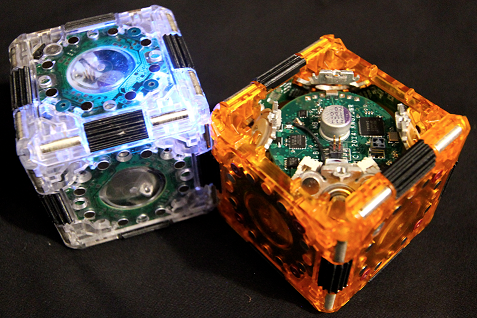
\includegraphics[width=3.4in]{Figures/cover.png}
%
%  \caption{M-Bocks modular robots with connections illuminated with onboard LEDs}
%
%  \label{fig:cover}
%\end{figure}
